\documentclass[a4paper, 12pt]{article}

\usepackage{graphicx}
\usepackage{longtable}
\usepackage[font=small,labelfont=bf]{caption}
\graphicspath{ {images/} }

\newcommand{\templates}{../../template}
\usepackage[a4paper, margin=2.5cm]{geometry}

\usepackage{enumitem}
\setlist[itemize]{noitemsep}
\setlist[enumerate]{noitemsep}

\let\oldpar\paragraph
\renewcommand{\paragraph}[1]{\oldpar{#1\\}\noindent}
\usepackage{graphicx}
\usepackage{hyperref}
\usepackage{makecell}

\newcommand{\settitolo}[1]{\newcommand{\titolo}{#1\\}}
\newcommand{\setprogetto}[1]{\newcommand{\progetto}{#1\\}}
\newcommand{\setcommittenti}[1]{\newcommand{\committenti}{#1\\}}
\newcommand{\setredattori}[1]{\newcommand{\redattori}{#1\\}}
\newcommand{\setrevisori}[1]{\newcommand{\revisori}{#1\\}}
\newcommand{\setresponsabili}[1]{\newcommand{\responsabili}{#1\\}}
\newcommand{\setversione}[1]{
	\ifdefined\versione\renewcommand{\versione}{#1\\}
	\else\newcommand{\versione}{#1\\}\fi
}
\newcommand{\setdestuso}[1]{\newcommand{\uso}{#1\\}}
\newcommand{\setdescrizione}[1]{\newcommand{\descrizione}{#1\\}}

\newcommand{\makefrontpage}{
	\begin{titlepage}
		\begin{center}

		
\includegraphics[width=0.4\textwidth]{../../template/WSWS-logos_transparent_crop}\\

		{\Large Winning Software Solution}\\[6pt]
		\href{mailto://winningsoftwaresolution@gmail.com}{winningsoftwaresolution@gmail.com}\\
		
		\ifdefined\progetto
		\vspace{1cm}
		{\Large\progetto}
		{\large\committenti}
		\else\fi
		
		\vspace{1.5cm}
		{\LARGE\titolo}
		
		\vfill
		
		\begin{tabular}{r | l}
		\multicolumn{2}{c}{\textit{Informazioni}}\\
		\hline
		
		\ifdefined\redattori
			\textit{Redattori} &
			\makecell[l]{\redattori}\\
		\else\fi
		\ifdefined\revisori
			\textit{Revisori} &
			\makecell[l]{\revisori}\\
		\else\fi
		\ifdefined\responsabili
			\textit{Respondabili} &
			\makecell[l]{\responsabili}\\
		\else\fi
		
		\ifdefined\versione
			\textit{Versione} & \versione
		\else\fi
		
		\textit{Uso} & \uso
		
		\end{tabular}
		
		\vspace{2cm}
		
		\ifdefined\descrizione
		Descrizione
		\vspace{6pt}
		\hrule
		\descrizione
		\else\fi
		\end{center}
	\end{titlepage}
}
\usepackage{hyperref}
\usepackage{array}
\usepackage{tabularx}

\def\vers#1-#2-#3-#4-#5\\{#1&#2&#3&#4&#5\\\hline}

\newcommand{\addversione}[5]{
	\ifdefined\versioni
		\let\old\versioni
		\renewcommand{\versioni}{#1&#2&#3&#4&#5\\\hline\old}
	\else
		\newcommand{\versioni}{#1&#2&#3&#4&#5\\\hline}
	\fi
}

\newcommand{\setversioni}[1]{\newcommand{\versioni}{#1}}

\newcommand{\makeversioni}{
	\begin{center}
		\begin{tabularx}{\textwidth}{|c|c|c|c|X|}
		\hline
		\textbf{Versione} & \textbf{Data} & \textbf{Persona} & \textbf{Attivtà} & \textbf{Descrizione} \\
		\hline
		\versioni
		\end{tabularx}
	\end{center}
	\clearpage
}

\settitolo{Specifiche Architetturali}
\setprogetto{ShopChain}
\setcommittenti{SyncLab}
\setredattori{Giovanni Cocco\\Elia Scandaletti\\Matteo Galvagni}
\setrevisori{Federico Marchi}
\setresponsabili{Giovanni Cocco}
\setdestuso{esterno}
\setdescrizione{
Architettura del progetto
}

\addversione{1.0.0}{23/02/2022}{Giovanni Cocco}{Redazione}{Creazione del documento}
\addversione{1.1.0}{03/04/2022}{E. Scandaletti, M. Galvagni}{Redazione}{Aggiunti dettagli dell'architettura}

\begin{document}

\makefrontpage

\makeversioni

\tableofcontents
\clearpage

\section{Introduzione}
\subsection{Scopo del documento}
Il documento illustra le scelte architetturali e illustra l'architettura.

\section{Riferimenti}
\subsection{Riferimenti normativi}
\begin{itemize}
    \item \underline{\href{https://www.math.unipd.it/~tullio/IS-1/2021/Progetto/C2.pdf}{Capitolato d'appalto C2}};
    \item \underline{\href{https://github.com/iota97/WinningSoftwareSolution/blob/main/public/interni/norme_di_progetto_v2.0.0.pdf}{Norme di Progetto}};
    \item \underline{\href{https://github.com/iota97/WinningSoftwareSolution/blob/main/public/esterni/verbali/2022_01_03_E.pdf}{Verbale esterno 2022/03/01}}.
\end{itemize}
\subsection{Riferimenti informativi}
\begin{itemize}
    \item \underline{\href{https://www.math.unipd.it/~tullio/IS-1/2021/Dispense/T09.pdf}{Progettazione Software - Materiale didattico del corso IS}};
    \item \underline{\href{https://www.math.unipd.it/~rcardin/swea/2022/Diagrammi\%20di\%20Sequenza.pdf}{Slide diagrammi di sequenza - Materiale didattico del corso IS}};
    \item \underline{\href{https://www.math.unipd.it/~rcardin/swea/2022/Software\%20Architecture\%20Patterns.pdf}{Slide design pattern architetturali - Materiale didattico del corso IS}};
    \item \underline{\href{https://www.math.unipd.it/~rcardin/swea/2021/Diagrammi\%20delle\%20Classi_4x4.pdf}{Slide diagrammi delle classi - Materiale didattico del corso IS}};
    \item \underline{\href{https://www.math.unipd.it/~rcardin/sweb/2022/L03.pdf}{Slide principi SOLID - Materiale didattico del corso IS}}.
\end{itemize}

\section{Tecnologie/Linguaggi/Librerie}

\subsection{Solidity}
\begin{itemize}
\item \textbf{Versione:} 0.8.13
\item \textbf{Documentazione:} \href{https://docs.soliditylang.org/en/v0.8.13/}{https://docs.soliditylang.org/en/v0.8.13/}
\end{itemize}

\subsection{Typescript}
\begin{itemize}
\item \textbf{Versione:} 4.6.3
\item \textbf{Documentazione:} \href{https://www.typescriptlang.org/docs/}{https://www.typescriptlang.org/docs/}
\end{itemize}

\subsection{Express}
\begin{itemize}
\item \textbf{Versione:} 4.17.2
\item \textbf{Documentazione:} \href{https://devdocs.io/express/}{https://devdocs.io/express/}
\end{itemize}

\subsection{MariaDB}
\begin{itemize}
\item \textbf{Versione:} 10.7.3
\item \textbf{Documentazione:} \href{https://mariadb.com/kb/en/documentation/}{https://mariadb.com/kb/en/documentation/}
\end{itemize}

\subsection{Python}
\begin{itemize}
\item \textbf{Versione:} 3.8
\item \textbf{Documentazione:} \href{https://docs.python.org/3.8/}{https://docs.python.org/3.8/}
\end{itemize}

\subsection{Web3}
\begin{itemize}
\item \textbf{Versione:} 1.7.1
\item \textbf{Documentazione:} \href{https://web3js.readthedocs.io/en/v1.7.1/}{https://web3js.readthedocs.io/en/v1.7.1/}
\end{itemize}

\subsection{MetaMask}
\begin{itemize}
\item \textbf{Versione:} 10.11.3
\item \textbf{Documentazione:} \href{https://docs.metamask.io/guide/}{https://docs.metamask.io/guide/}
\end{itemize}

\section{Architettura generale}
Il progetto si compone di 4 macro parti:
\begin{itemize}
\item Server
\item Smart contract
\item Web app
\item Script di messa in vendita
\end{itemize}
\subsection{Server}
Realizzato in typescript con express come modulo http e MariaDB come database SQL.
Si divide in 2 parti principali: la persistenza e il server web.
\subsubsection{Persistenza}
Si occupa di gestire i dati delle transazioni.\\\\
Si collega allo smart contract attraverso un websocket fornito da moralis.io.\\
Rimane in ascolto degli eventi dello smart contract e
aggiorna il database SQL di conseguenza.\\
Tiene sempre traccia dell'ultimo blocco da cui ha ricevuto un evento
e all'avvio recupera tutti gli eventi arretrati partendo da quest'ultimo blocco.\\\\
I dati nel database SQL vengono forniti al frontend.\\\\
Notare come è molto oneroso
effettuare query sui dati in block chain in quanto non sono disponibili strutture dati adeguate.\\
Questa soluzione ci permette una maggiore flessibilità e apertura a modifiche future quali aggiungere query specifiche.\\\\
Inoltre il contratto una volta pubblicato non può essere modificabile al fine di garantire la trasparenza ed è quindi cruciale
che il codice di quest'ultimo sia semplice ed affidabile.
\subsubsection{Server Web}
Riceve le richieste HTTP dalla rete e risponde con le pagine della Web app.

\subsection{Smart contract}
Realizzato in solidity e pubblicato sulla rete Polygon tiene traccia delle transazioni; gestisce la logica e la sicurezza di esse.\\\\
Per gestire il timer che fa scadere le transazioni si usa il servizio Upkeep di ChainLink.\\
Uno smart contract non esegue operazioni se non viene chiamato, per realizzare un timer si realizzano delle funzioni che
eseguono le operazioni necessarie se è passato abbastanza tempo. Un upkeeper chiama automaticamente queste funzioni dall'esterno a intervalli di tempo prefissato.

\subsection{Web app}
Fornita all'utente tramite il server web fornisce la logica lato client.\\
Tramite MetaMask l'utente interagisce direttamente col contratto.\\\\
In caso di utenti mobile reindirizza tramite deep link per aprire la pagine sull'app di Metamask.\\\\
I deep link vengono usati anche per il QR code di ricezione del pacco.\\
Possono essere scansionati sia da dentro l'app di MetaMask che dalla fotocamera del cellulare.

\subsection{Script di messa in vendita}
Usato dall'e-commerce per inserire prodotti in vendita in blockchain al fine di verificare che il prezzo sia corretto al momento della vendita.
Realizzato in python per flessibilità, si connette alla block chain tramite moralis.io.
\newpage
\section{Dettagli architettura}
\subsection{Server}
\subsubsection{Diagramma delle classi}
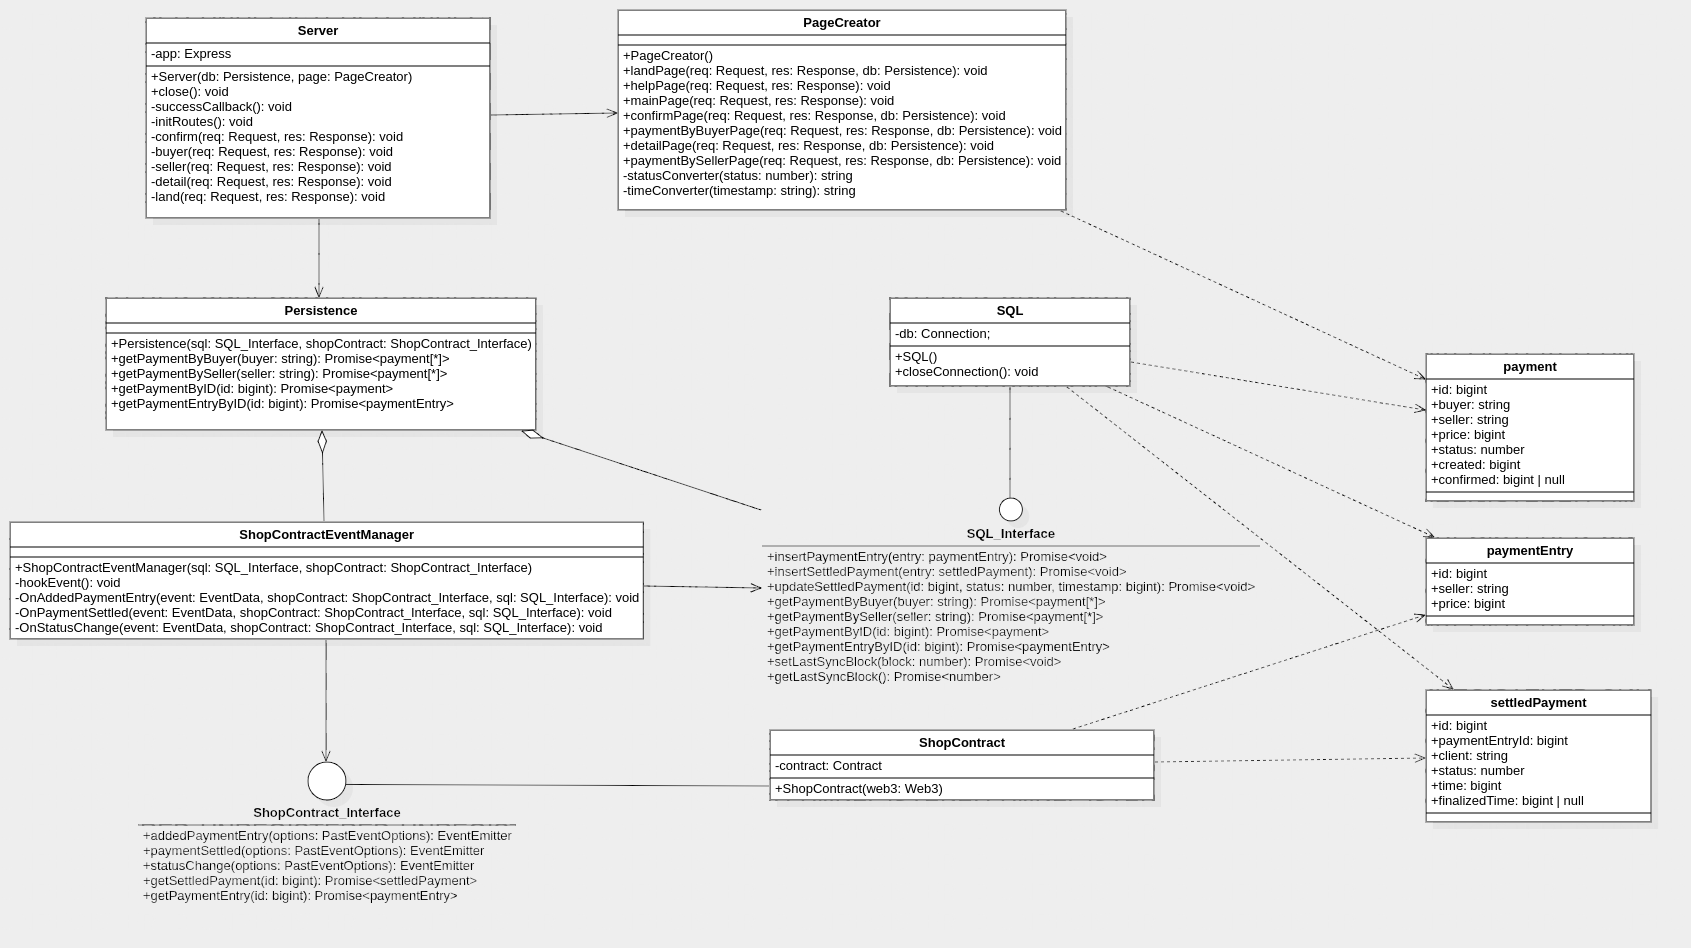
\includegraphics[width=1.0\textwidth]{server_class}
\captionof{figure}{Diagramma delle classi del server}
\paragraph{Commenti}
La classe ShopContract andrà a interfacciarsi con il contratto in blockchain.\\
La classe PageCreator andrà a interfacciarsi con la WebApp.
\subsubsection{Design pattern: Constructor injection}
\paragraph{Descrizione}
Le dipendenze sono tracciate e passate agli oggetti tramite il costruttore.
\paragraph{Motivazioni}
Facilita il tracciamento delle dipendenze e agevola il mocking in fase di test.
\subsubsection{Schema DB}
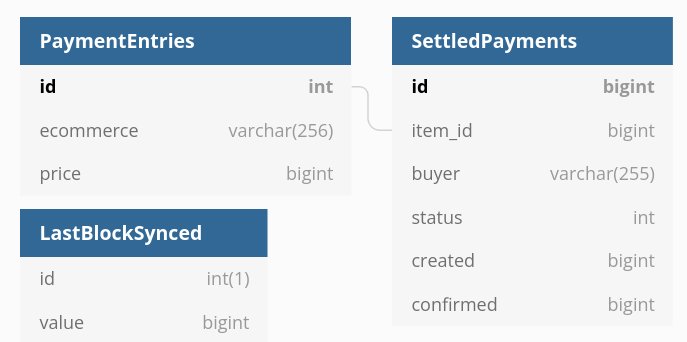
\includegraphics[width=1.0\textwidth]{db}
\captionof{figure}{Schema del DB relazionale}
\paragraph{Commenti}
Schema delle tabelle del database.\\
\textbf{LastSyncedBlock} contiene una sola riga con \textit{id} 0 con il valore dell'ultimo blocco sincronizzato.

\newpage
\subsection{Smart contract}
\subsubsection{Diagramma delle classi}
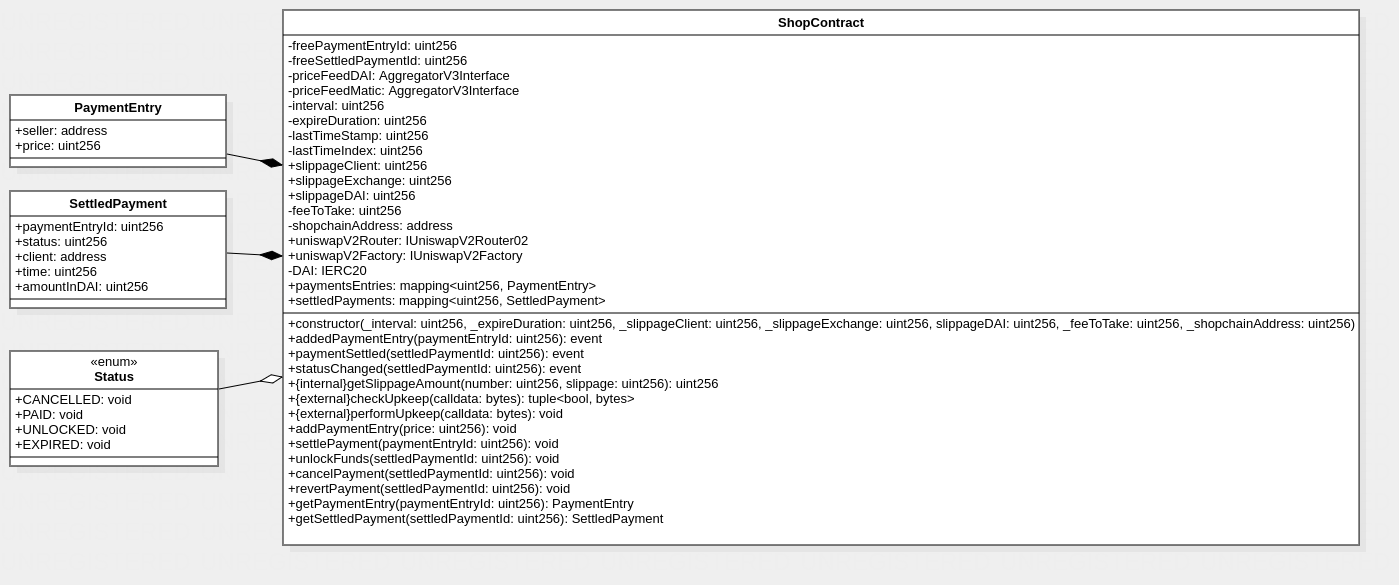
\includegraphics[width=1.0\textwidth]{contract}
\captionof{figure}{Diagramma delle classi del contratto}
\paragraph{Commenti}
In Solidity esistono due particolari visibilità di funzione che differiscono da quelle normali: \textit{internal} ed \textit{external}.
Una funzione \textit{internal} può essere chiamata solo dal contratto in cui è dichiarata e da contratti derivanti.
È l'equivalente di \textit{protected}.
Una funzione \textit{external} può essere chiamata solo dall'esterno e non all'interno del contratto stesso.
\subsubsection{Lista dei metodi}
\begin{itemize}
    \item \textbf{constructor(\_interval: uint256, \_expireDuration: uint256, \_slippageClient: uint256, \_slippageExchange: uint256, \_slippageDAI: uint256, \_feeToTake: uint256, \_shopchainAddress: address): void}
    \\Imposta l'intervallo di controllo per aggiornamenti e l'intervallo di scadenza.
    Imposta gli slippage, la percentuale di fee da trattenere e l'address a cui inviarla.
    Imposta router e factory dell'exchange su cui convertire Matic in DAI.\\
    \item \textbf{checkUpkeep(calldata: bytes): (upkeepNeeded: bool, memory: bytes)}
    Se chiamata, restituisce tramite \textit{upkeepNeeded} se è passato l'intervallo di tempo minimo dall'ultimo upkeep e dunque se è necessario eseguirne un altro.\\
    \item \textbf{performUpkeep(calldata: bytes): void}
    Controlla se l'intervallo di tempo minimo per ogni upkeep è passato, se è così scorre dall'ultima transazione vista alla più recente transazione che abbia superato la durata massima senza sblocco dei fondi
    e restituisce il denaro all'indirizzo del cliente.\\
    \item \textbf{addPaymentEntry(price: uint256): void}
    Aggiunge un'entry di pagamento alla relativa mappa.\\
    \item \textbf{settlePayment(paymentEntryId: uint256): void}
    Completa il pagamento dato l'id di un pagamento aperto, eseguendo i necessari controlli e aggiungendo un nuovo pagamento completato alla relativa mappa.\\
    \item \textbf{unlockFunds(settledPaymentId: uint256): void}
    Dato l'id di un pagamento completato, se chiamata dal cliente originale e dopo necessari controlli sblocca i fondi che vengono inviati all'indirizzo del venditore.\\
    \item \textbf{cancelPayment(settledPaymentId: uint256): void}
    Se il venditore avesse necessità di annullare una transazione dopo il pagamento da parte del cliente, questa funzione si occuperà di restituire il denaro al cliente.\\
    \item \textbf{revertPayment(settledPaymentId: uint256): void}
    Se il servizio di UpKeep dovesse smettere di funzionare per qualsiasi motivo, questa funzione consente al cliente di ottenere un rimborso manualmente qualora il pacco non sia arrivato dopo l'intervallo prefissato.\\
    \item \textbf{getPaymentEntry(paymentEntryId: uint256): PaymentEntry}
    Ritorna l'oggetto rappresentante un'entry di pagamento aperta da un venditore.\\
    \item \textbf{getSettledPayment(settledPaymentId: uint256): SettledPayment}
    Ritorna l'oggetto rappresentante un pagamento completato da un cliente relativo ad un'entry di pagamento di un venditore.\\

\end{itemize}
\subsubsection{Design pattern: Oracle}
\paragraph{Descrizione}
Le informazioni sul reale valore di una valuta sono fornite da un oracolo.
\paragraph{Motivazioni}
Per evitare manipolazioni temporanee del valore della valuta stabile utilizzata si utilizza il valore fornito da ChainLink.
ChainLink restituisce la media del valore di una valuta tra più fornitori, evitando manipolazioni di un singolo fornitore.
\subsubsection{Design pattern: Access restriction}
\paragraph{Descrizione}
La chiamata di alcune funzioni è ristretta ad alcune tipologie di utenti.
\paragraph{Motivazioni}
È necessario mantenere una distinzione tra cliente e venditore all'interno del contratto.
Il venditore non potrà chiamare funzioni riservate al cliente (per esempio, sbloccandosi i fondi) e viceversa.
\subsubsection{Design pattern: Guard check}
\paragraph{Descrizione}
L'input fornito alle funzioni è validato prima di essere processato, annullando la transazione se non valido.
\paragraph{Motivazioni}
Alcune funzioni richiedono il passaggio in input di un ID.
Deve essere controllato che tale ID esista prima di continuare le operazioni.

\subsubsection{Testing}
Per testare il contratto si utilizza la suite Truffle (usata anche per compilazione e deployment).
Al fine di includere nei test di unità la copertura del codice, viene utilizzato il plugin solidity-coverage alla versione 0.6.3 (documentazione al link \href{https://github.com/sc-forks/solidity-coverage/tree/0.6.x-final#solidity-coverage}{https://github.com/sc-forks/solidity-coverage/tree/0.6.x-final#solidity-coverage}).\\
Il plugin clona la blockchain di test Mumbai di Polygon e la esegue in locale, per poi effettuarvici il deployment del contratto ed eseguire i test.\\
Di comune accordo col Proponente i test che richiedono il mocking completo di altri contratti non sono stati eseguiti visto l'alto costo di implementazione e la bassa utilità.

\newpage
\subsection{Web app}
\subsubsection{Diagramma delle classi}
Non sono presenti classi. Questo perché introdurre delle classi avrebbe aumentato la complessità del codice, a fronte di vantaggi irrisori. Questo perché la web app è molto semplice ed una mera interfaccia asincrona per la comunicazione col contratto in blockchain.
\subsubsection{Lista dei metodi}
Nessuno dei seguenti metodi prevede alcuna verifica sull'identità dell'utente o sulla validità delle richieste fatte. Questo perché la web app serve solo a fare da interfaccia per la blockchain che è pubblica per definizione. Tutta la parte di sicurezza è implementata nel contratto. Inoltre, essendo lo script eseguito lato client, sarebbe facile per un attaccante bypassare qualsiasi controllo.
\begin{itemize}
    \item \textbf{mobileCheck(): boolean} Controlla se sta venendo usato un dispositivo mobile.\\
    \item \textbf{toggleMenu(): void} Mostra o nasconde il menu nella versione mobile dell'app.\\
    \item \textbf{setGetParameter(paramName: string, paramValue: string): void} Imposta un dato parametro GET nella barra dell'URL del browser.\\
    \item \textbf{findGetParameter(parameterName: string): string} Ritorna un dato parametro GET dall'URL corrente.\\
    \item \textbf{handleNewChain(id: string): void} Funzione utilizzata per gestire il cambio di blockchain a cui è collegato MetaMask.\\
    \item \textbf{handleNewAccounts(newAccounts: string[]): void} Funzione utilizzata per gestire il cambio di wallet utilizzati in MetaMask.\\
    \item \textbf{async isMetamaskConnected(): boolean} Controlla se MetaMask è connesso a un wallet.\\
    \item \textbf{showSellerButton(): void} Nella parte di web app relativa al venditore, mostra il bottone di annullamento dell'ordine insieme al QR code.\\
    \item \textbf{showBuyerButton(): void} Nella parte di web app relativa all'acquirente, mostra il bottone di sblocco manuale del pagamento.\\
    \item \textbf{showContents(): void} Nasconde i pop-up e mostra il contenuto della pagina.\\
    \item \textbf{updateMenuLink(): void} Aggiorna i link nel menù in modo che puntino alle pagine relative al wallet attualmente collegato.\\
    \item \textbf{async onMetamaskConnected(): void} Procedura asincrona che viene eseguita alla connessione di MetaMask a un wallet.\\
    \item \textbf{onClickInstall(): void} Procedura per l'installazione di MetaMask.\\
    \item \textbf{async onClickConnect(): void} Procedura per la connessione a MetaMask.\\
    \item \textbf{async onClickOpenMetaMask(): void} Procedura per aprire la web app nell'applicazione mobile di MetaMask.\\
    \item \textbf{isMetaMaskInstalled(): boolean} Controlla se MetaMask è installato.\\
    \item \textbf{askForInstall(): void} Mostra un pop-up per chiedere all'utente di installare MetaMask.\\
    \item \textbf{askToConnect(): void} Mostra un pop-up per chiedere all'utente di collegare il proprio wallet a MetaMask.\\
    \item \textbf{async initialize(): void} Funzione di inizializzazione che verifica se MetaMask è installato e collegato a un wallet e, in caso negativo, mostra i rispettivi pop-up per guidare l'utente nella risoluzione del problema.\\
    \item \textbf{closePop(e: Event): void} Procedura per chiudere il pop-up dato.\\
    \item \textbf{checkChainID(): boolean} Controlla che MetaMask sia collegata alla stessa blockchain del contratto.\\
    \item \textbf{showStatus(id: int): void} Mostra il pop-up corrispondente all'esito della transazione in corso o appena effettuata.\\
    \item \textbf{onClickSettlePayment(): void} Procedura per invocare il metodo del contratto settledPayment.\\
    \item \textbf{onCancelPayment(): void} Procedura per invocare il metodo del contratto cancelPayment.\\
    \item \textbf{onClickUnlockFunds(): void} Procedura per invocare il metodo del contratto unlockFunds.\\
\end{itemize}
\subsubsection{Design pattern: Nessuno}
\paragraph{Descrizione}
Non è stato adottato alcun design pattern.
\paragraph{Motivazioni}
Adottare pattern architetturali avrebbe richiesto un costo ben superiore ai benefici. Questo perché la web app è molto semplice ed una mera interfaccia asincrona per la comunicazione col contratto in blockchain.

\subsection{Script di messa in vendita}
\subsubsection{sell\_item}
\textbf{Parametri}\\
price: float - il prezzo in dollari della entry di pagamento.\\\\
\textbf{Valore Restituito}\\
entry id: int - l'id dell'entry inserita in blockchain (-1 in caso di errore).\\\\
\textbf{Comportamento}\\
Il metodo inserisce una nuova entry di pagamento in blockchain con il prezzo specificato.\\
Sia in caso si successo che di errore tutte le informazioni vengono salvate nel file \textit{sell.log}.

\section{Diagrammi di sequenza}
\subsection{Inizializzazione server web}
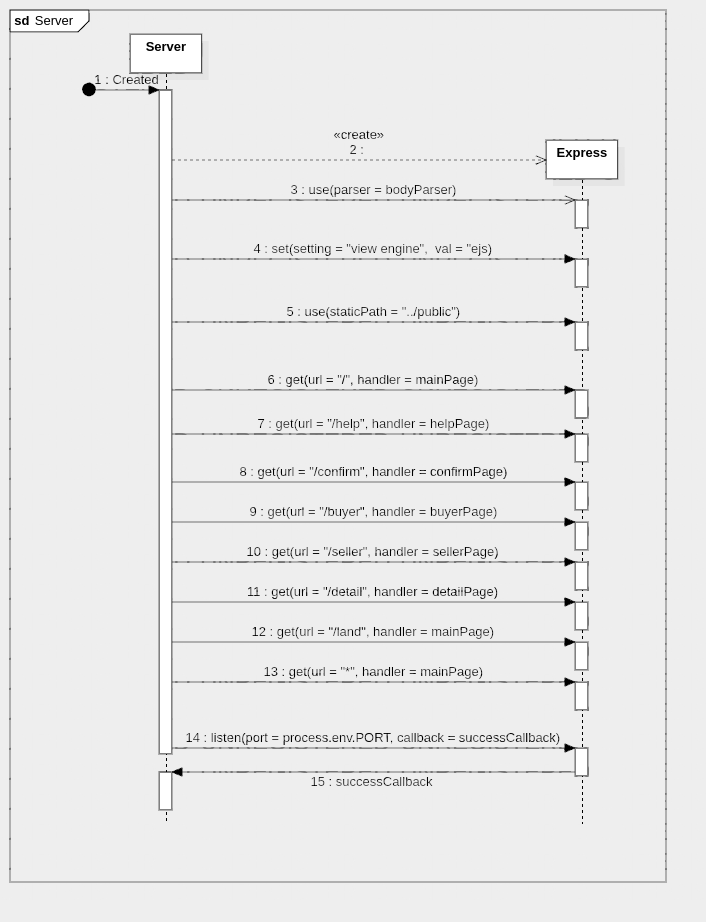
\includegraphics[width=1.0\textwidth]{server}
\captionof{figure}{Diagramma di sequenza dell'inizializzazione del server}
\paragraph{Commenti}
Mostra l'inizializzazione delle routes per express.

\subsection{Ascolto eventi del contratto}
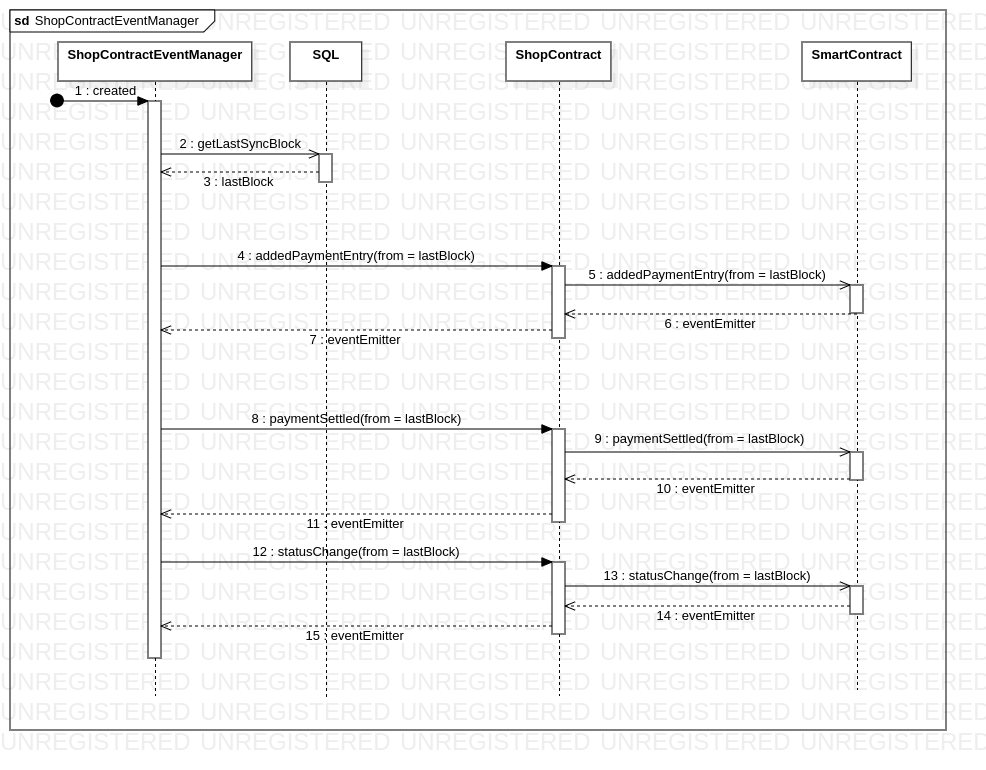
\includegraphics[width=1.0\textwidth]{shopContractEventManager}
\captionof{figure}{Diagramma di sequenza dell'ascolto degli eventi}
\paragraph{Commenti}
Mostra la sottoscrizione degli eventi del contratto.

\subsection{Nuovo oggetto in vendita}
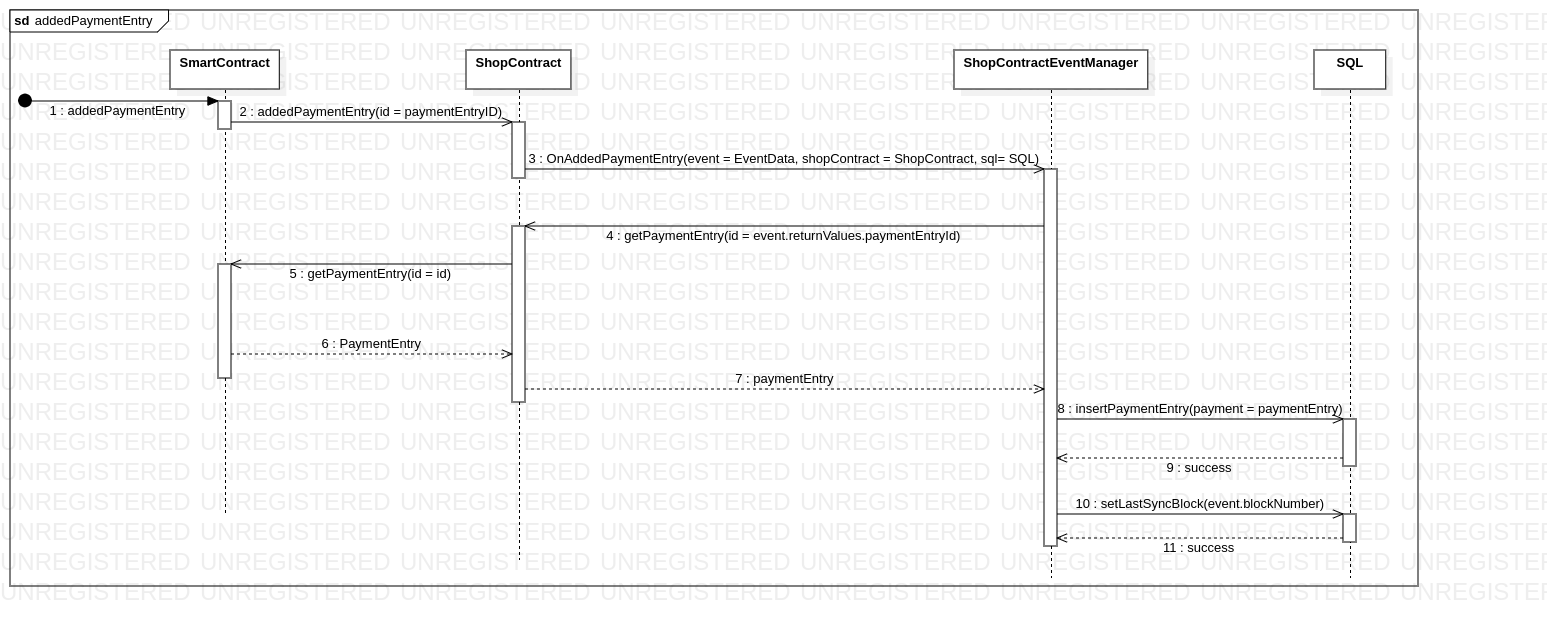
\includegraphics[width=1.0\textwidth]{addedPaymentEntry}
\captionof{figure}{Diagramma di sequenza di un nuovo oggetto in vendita}
\paragraph{Commenti}
Mostra cosa succede quando viene inserita una nuova entry di pagamento da parte di un e-commerce.

\subsection{Nuova transazione}
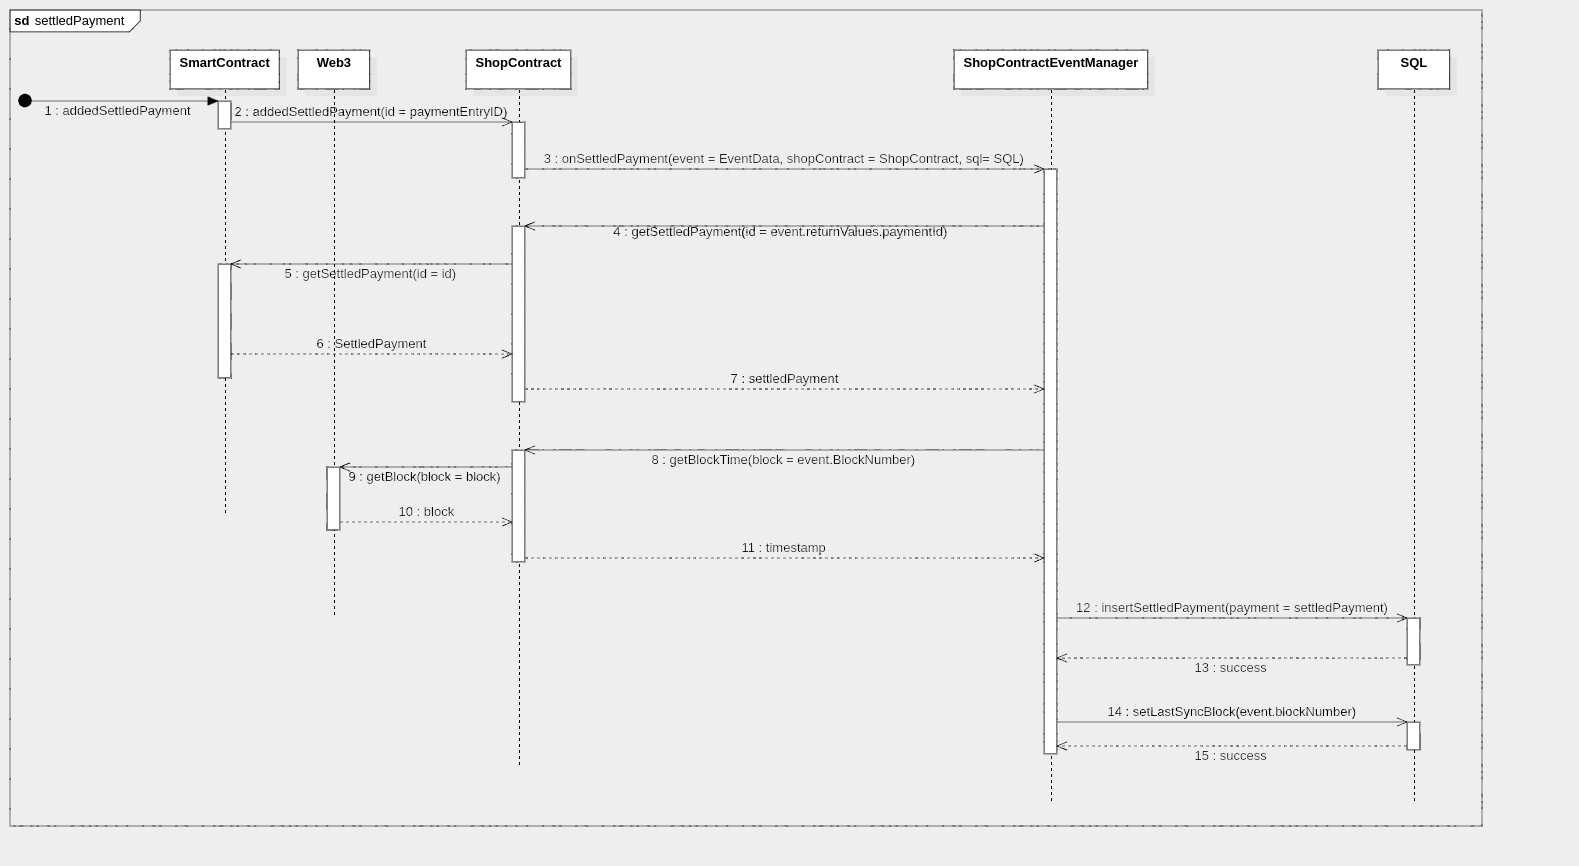
\includegraphics[width=1.0\textwidth]{settledPayment}
\captionof{figure}{Diagramma di sequenza di una nuova transazione}
\paragraph{Commenti}
Mostra cosa succede quando viene creata una nuova transazione.

\subsection{Cambio di stato di una transazione}
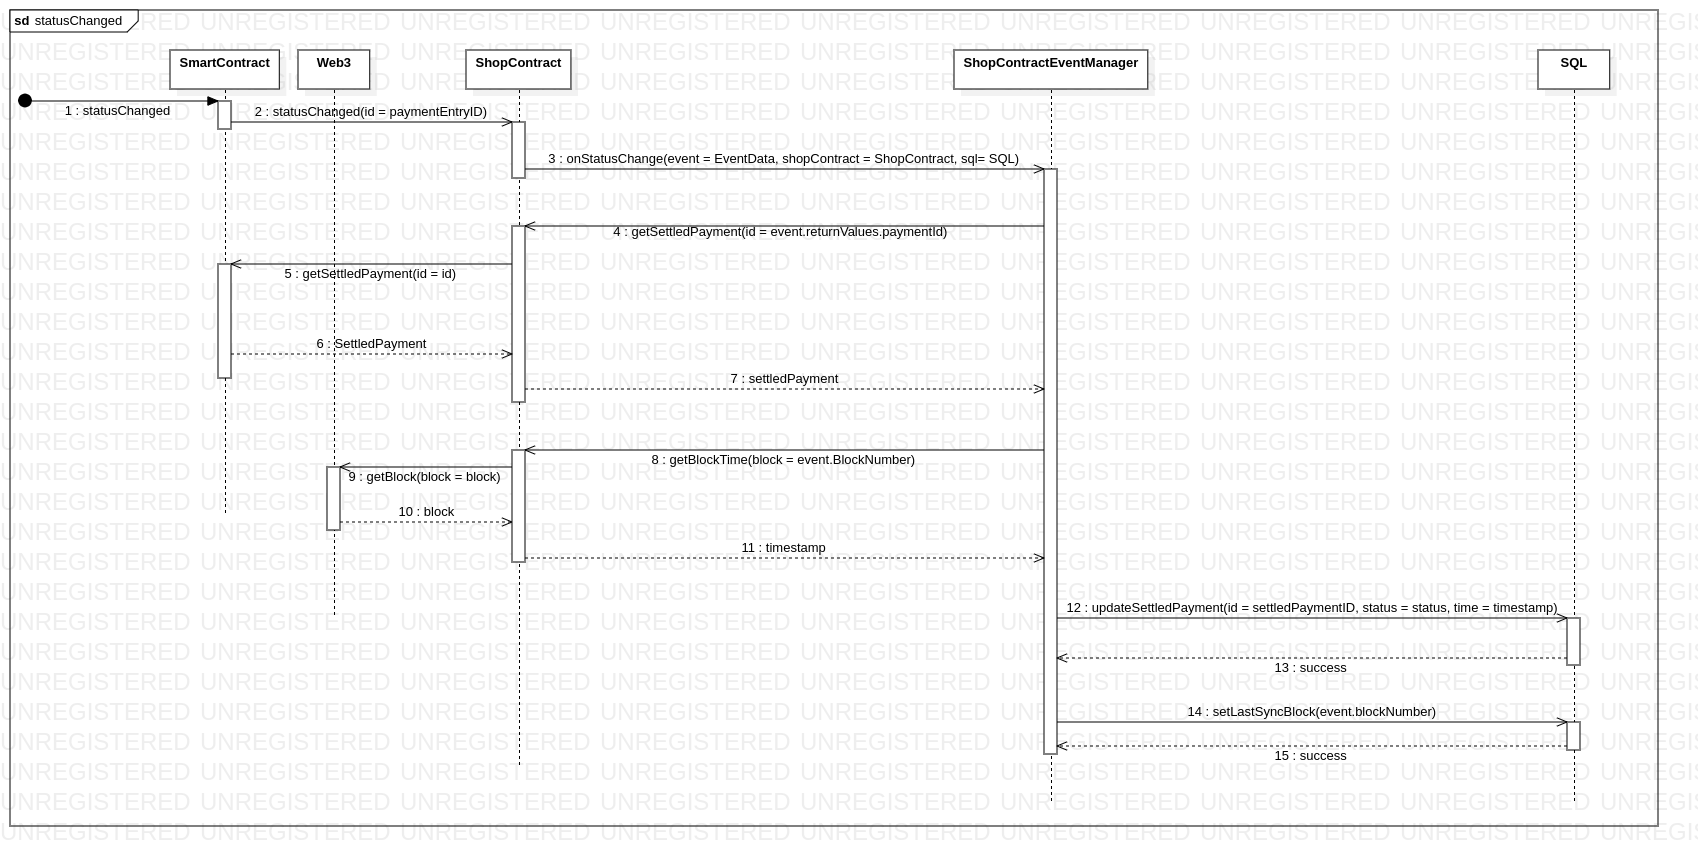
\includegraphics[width=1.0\textwidth]{statusChanged}
\captionof{figure}{Diagramma di sequenza del cambio di stato di una transazione}
\paragraph{Commenti}
Mostra cosa succede quando una transazione cambia di stato.

\subsection{Pagina transazioni in entrata}
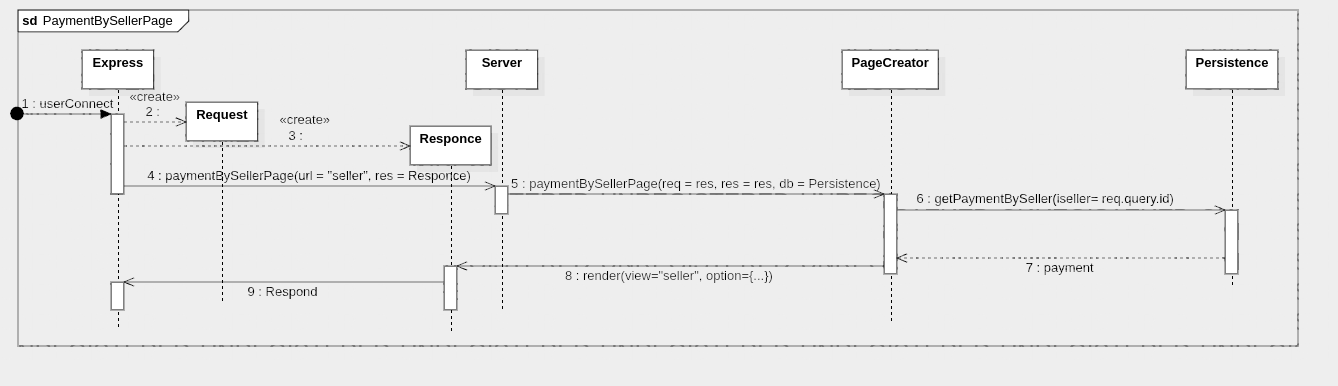
\includegraphics[width=1.0\textwidth]{paymentBySellerPage}
\captionof{figure}{Diagramma di sequenza della richiesta della pagina delle transazioni in entrata}
\paragraph{Commenti}
Mostra cosa succede quando un utente richiede la pagina delle transazione in entrata.\\
Le altre pagine utilizzano lo stesso modello e dunque si preferisce evitare diagrammi di sequenza ridondanti.

\end{document}